% Un articolo scritto con LaTeX
\documentclass[a4paper,11pt]{article}
\usepackage{graphicx}
\usepackage[T1]{fontenc} % codifica dei font in uscita
\usepackage[utf8]{inputenc} % lettere accentate da tastiera
\usepackage[italian]{babel} % lingua principale del documento
\usepackage{url}
\usepackage [a4paper, top=2.5cm, bottom=2.5cm, left=1.5cm, right=1.5cm, bindingoffset=8mm] {geometry}

% inizio documento

\usepackage{graphicx}
\begin{document}
\begin{center}
\textbf{\huge Esperienza VI} \\ \vspace{10pt}
\large Alberini Giacomo \\ Bassini Luigi \\ Michele Pedrotti\\ Trevisson Nicola 
\end{center}
\section{Scopo dell'esperienza}
Lo scopo di questa esperienza è quello di misurare la conduttanza di vari tubi con diametri e lunghezze diversi in regimi di flusso differenti. Successivamente le conduttanze ottenute sperimentalmente verranno confrontate con i valori attesi calcolati tenendo conto del tipo di regime di flusso. 
\section{Misura della Conduttanza}

Per calcolare la conduttanza si è reso necessario l'uso di una pompa da vuoto, due pirani (con relativa strumentazione di misura), una valvola a spillo (già tarata in precedenza) e vari tubi con lunghezze e diametri differenti.

	
\begin{center} 
\begin{figure}[htpd]
\hspace{120pt}
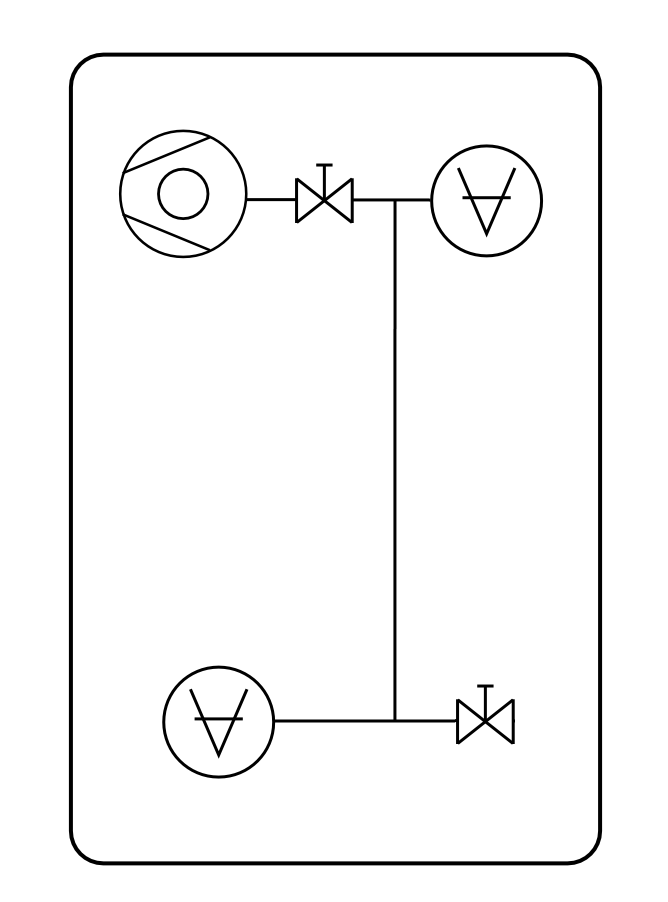
\includegraphics[scale=0.5]{schema_finale.png}
\end{figure}
\end{center}

Nello schema soprastante, per semplicità, i vari tubi sono indicati dalla linea retta verticale tra i due T che collegano i pirani.
Per ottenre il valore di conduttanza a differenti regimi di flusso, opportunamente creati tramite la manipolazione della valvola a spillo, si sono utilizzati i due pirani. Essi hanno permesso di rilevare i valori di pressione in testa e in coda al tubo sotto analisi. L'andamento della pressione è stato monitorato tramite un software che riportava in tempo reale i valori di pressione in un grafico. Questo grafico, aggiornato in tempo reale, ha reso possibile l'osservazione del momento in cui la pressione si stabilizzava dopo un cambiamento come ad esempio l'apertura e la chiusura della valvola. Una volta stabilizzata la pressione si è proceduto all'annotazione del valore di pressione corrispondente al numero di tacche di apertura della valvola a spillo (dal vuoto nel tubo per poi salire da 4 a 8 giri e ritorno).
Una volta ottenuti tutti i dati relativi ad ogni tubo a nostra disposizione si passa al calcolo della conduttanza. Per fare questo è necessario utilizzare i dati di flusso delle precedenti esperienze relativi alla valvola a spillo. Noto il flusso Q della valvola a spillo e nota la differenza di pressione fra testa e coda $\delta p$ si può ricavare la conduttanza C tramite l'ugualianza $ C = \frac{Q}{\Delta P} $.\\
I valori ricavati sperimentalmente sono poi confrontati con quelli di conduttanza teorica attesi.
Per poter calcolare i valori di conduttanza teorica è necessario conoscere il tipo di regime del flusso.\\
Questi regimi di flusso sono legati al regime di vuoto per cui i primi tre (viscoso laminare, viscoso intermedio, viscoso turbolento) appartengono ad un regime di basso vuoto, il regime transitorio appartiene al regime di medio vuoto e il regime molecolare è relativo ai sistemi di alto vuoto e ultra alto vuoto.\\
Nel nostro caso si passa da un regime di basso vuoto ad un regime di medio vuoto. Ogni regime presenta una formula differente per il calcolo della conduttanza teorica.
Per un corretto calcolo del valore teorico di conduttanza si utilizza la seguente formula:
$$ Re=\frac{4}{\pi \eta d}\frac{M}{RT}Q$$
Dove $ \eta $ è la viscosità dinamica del fluido(alla temperatura di 20$^\circ C$), $ d $ è il diametro della canalizzazione e $ Q $ è il flusso precedentemente trovato (riportato nella seguente tabella).
\begin{center}
\begin{tabular}{|c|c|}
\hline $Tacche$ & $Q\pm\delta Q$ [$Pa\cdot m^{3}$$\cdot s^{-1}$] \\ 

\hline 4 & 2.97$\cdot10^{-5}$$\pm 2\cdot10^{-7}$ \\ 
\hline 5 & 2.06$\cdot10^{-4}$$\pm 9\cdot10^{-7}$ \\ 
\hline 6 & 3.18$\cdot10^{-3}$$\pm 1\cdot10^{-5}$ \\ 
\hline 7 & 4.93$\cdot10^{-2}$$\pm 2\cdot10^{-4}$ \\ 
\hline 8 & 3.00$\cdot10^{-1}$$\pm 1\cdot10^{-3}$ \\ 
\hline 
\end{tabular}
\end{center}
In base al regime teorico all'interno del tubo si andrà ad utilizzare una delle due seguenti formule. La prima è adatta al calcolo della conduttanza teorica nel regime laminare mentre la seconda è adatta al calcolo della conduttanza nel regime molecolare.
$$C_{lam}=1350\frac{\bar{P}d^4}{l}[m^3/s]$$
$$C_{molec}=120\frac{d^3}{l}[m^3/s]$$
 
Nelle seguenti tabelle si riportano i risultati ottenuti.\\
 

\begin{center} 
\begin{tabular}{|c|c|c|c|}
\hline Apertura valvola & $C_{lab} [m^3/s]$ & Regime di flusso & $C_{teo} [m^3/s]$ \\ 
\hline 4 & 0.0015 $\cdot10^{-4}\pm 0.0006\cdot10^{-4}$ & transitorio & 0.0046$\cdot10^{-3}\pm 0.0003\cdot10^{-3}$ \\ 
\hline 5 & 0.010$\cdot10^{-4}\pm 0.007\cdot10^{-4}$ & transitorio & 0.0055$\cdot10^{-3}\pm 0.0006\cdot10^{-3}$ \\ 
\hline 6 & 0.06$\cdot10^{-4}\pm 0.01\cdot10^{-4}$ & transitorio & 0.011$\cdot10^{-3}\pm 0.001\cdot10^{-3}$ \\
\hline 7 & 0.24$\cdot10^{-4}\pm 0.05\cdot10^{-4}$ & laminare 10.4$\pm0.1$ & 0.045$\cdot10^{-3}\pm 0.003\cdot10^{-3}$ \\
\hline 8 & 0.68$\cdot10^{-4}\pm 0.09\cdot10^{-4}$ & laminare 63$\pm1$ & 0.10$\cdot10^{-3}\pm 0.01\cdot10^{-3}$ \\ 
\hline 
\end{tabular}\\
\vspace{5pt}
Tubo di lunghezza $8m$ e diametro $4mm$ .
\\
\vspace{15pt}
\begin{tabular}{|c|c|c|c|}
\hline Apertura valvola & $C_{lab} [m^3/s]$ & Regime di flusso & $C_{teo} [m^3/s]$ \\ 
\hline 4 & 0.0011$\cdot10^{-3}\pm 0.0001\cdot10^{-3}$ & transitorio & 0.0070$\cdot10^{-3}\pm 0.0008\cdot10^{-3}$ \\ 
\hline 5 & 0.0059$\cdot10^{-3}\pm 0.0006\cdot10^{-3}$ & transitorio & 0.0086$\cdot10^{-3}\pm 0.0007\cdot10^{-3}$ \\ 
\hline 6 & 0.023$\cdot10^{-3}\pm 0.0002\cdot10^{-3}$ & transitorio & 0.032$\cdot10^{-3}\pm 0.0004\cdot10^{-3}$ \\
\hline 7 & 0.095$\cdot10^{-3}\pm 0.008\cdot10^{-3}$ & laminare 10.4$\pm0.1$ & 0.13$\cdot10^{-3}\pm 0.01\cdot10^{-3}$ \\
\hline 8 & 0.24$\cdot10^{-3}\pm 0.02\cdot10^{-3}$ & laminare 63$\pm1$ & 0.40$\cdot10^{-3}\pm 0.05\cdot10^{-3}$ \\ 
\hline 
\end{tabular}\\
\vspace{5pt}
Tubo di lunghezza $80cm$ e diametro $4mm$.
\\
\vspace{15pt}
\begin{tabular}{|c|c|c|c|}
\hline Apertura valvola & $C_{lab} [m^3/s]$ & Regime di flusso & $C_{teo} [m^3/s]$ \\ 
\hline 4 & 0.0070$\cdot10^{-4}\pm 0.0006\cdot10^{-4}$ & transitorio & 0.0014$\cdot10^{-3}\pm 0.0001\cdot10^{-3}$ \\ 
\hline 5 & 0.027$\cdot10^{-4}\pm 0.003\cdot10^{-4}$ & transitorio & 0.0026$\cdot10^{-3}\pm 0.0002\cdot10^{-3}$ \\ 
\hline 6 & 0.095$\cdot10^{-4}\pm 0.009\cdot10^{-4}$ & laminare 1.1$\pm0.1$ & 0.011$\cdot10^{-3}\pm 0.001\cdot10^{-3}$\\
\hline 7 & 0.35$\cdot10^{-4}\pm 0.03\cdot10^{-4}$ & lamianre 16$\pm1$ & 0.049$\cdot10^{-3}\pm 0.005\cdot10^{-3}$ \\
\hline 8 & 0.94$\cdot10^{-4}\pm 0.09\cdot10^{-4}$ & laminare 102$\pm9$ & 0.12$\cdot10^{-3}\pm 0.01\cdot10^{-3}$ \\ 
\hline 
\end{tabular}\\
\vspace{5pt}
Tubo di lunghezza $80cm$ e diametro $2.5mm$.
\\
\vspace{15pt}
\begin{tabular}{|c|c|c|c|}
\hline Apertura valvola & $C_{lab} [m^3/s]$ & Regime di flusso & $C_{teo} [m^3/s]$ \\ 
\hline 4 & 0.0007$\cdot10^{-4}\pm 0.0001\cdot10^{-4}$ & transitorio & 0.012$\cdot10^{-4}\pm 0.001\cdot10^{-4}$ \\ 
\hline 5 & 0.0046$\cdot10^{-4}\pm 0.0004\cdot10^{-4}$ & transitorio & 0.014$\cdot10^{-4}\pm 0.001\cdot10^{-4}$ \\ 
\hline 6 & 0.024$\cdot10^{-4}\pm 0.002\cdot10^{-4}$ & laminare 1.1$\pm0.1$ & 0.042$\cdot10^{-4}\pm 0.004\cdot10^{-4}$ \\
\hline 7 & 0.10$\cdot10^{-4}\pm 0.01\cdot10^{-4}$ & laminare 16$\pm1$ & 0.15$\cdot10^{-4}\pm 0.01\cdot10^{-4}$ \\
\hline 8 & 0.10$\cdot10^{-4}\pm 0.01\cdot10^{-4}$ & laminare 102$\pm9$ & 0.96$\cdot10^{-4}\pm 0.09\cdot10^{-4}$ \\ 
\hline 
\end{tabular}\\
\vspace{5pt}
Tubo di lunghezza $8m$ e diametro $2.5mm$.
\\
\vspace{15pt}
\begin{tabular}{|c|c|c|c|}
\hline Apertura valvola & $C_{lab} [m^3/s]$ & Regime di flusso & $C_{teo} [m^3/s]$ \\ 
\hline 4 & 1.2$\cdot10^{6}\pm 0.1\cdot10^{6} $ & transitorio & 0.035 $\cdot10^{-3}\pm 0.003\cdot10^{-3}$ \\ 
\hline 5 & 0.20$\cdot10^{6}\pm 0.02\cdot10^{6}$ & transitorio & 0.042 $\cdot10^{-3}\pm 0.004\cdot10^{-3}$\\ 
\hline 6 & 0.026$\cdot10^{6}\pm 0.002\cdot10^{6}$ & transitorio & 0.091$\cdot10^{-3}\pm 0.009\cdot10^{-3}$ \\
\hline 7 & 0.0043$\cdot10^{6}\pm 0.0004\cdot10^{6}$ & laminare 5.2$\pm0.5$ & 0.32$\cdot10^{-3}\pm 0.03\cdot10^{-3}$ \\
\hline 8 & 0.0011$\cdot10^{6}\pm 0.0001\cdot10^{6}$ & laminare 31$\pm3$ & 0.92$\cdot10^{-3}\pm 0.09\cdot10^{-3}$ \\ 
\hline 
\end{tabular}\\
\vspace{5pt}
Composizione di due tubi di acciaio in serie con tre vacuometri in tre punti dell'impianto, uno in testa, uno in coda e uno in posizione intermedia fra i due tubi.
\vspace{10pt}
\end{center}
In quest'ultima tabella, relativa ai tubi in metallo collegati in serie, è stata inserita l'impedenza al posto della conduttanza poichè questa è stata calcolata per i singoli tubi e quindi si è resonecessario l'utilizzo delle seguenti formule: $$Z=\sum_{i=1}^{n}Z_i $$ \begin{center}equivalente a\end{center}  $$ 1/C=\sum_{i=1}^{n}1/C_i $$
Queste ci hanno permesso di calcolare l'impedenza di due tubi distinti uniti tramite un raccordo T. Su uno dei capi del raccordo era collegato un vacuometro pirani necessario alla misura della pressione intermedia dell'apparato. Questo valore di pressione, noto il flusso della nostra valvola a spillo, ci ha permesso di calcolare, riducendo l'errore, la conduttanza di un tubo senza considerare l'altro.

Nei conti si è tenuto in considerazione per la viscosità dinamica e per la fomula $ M/RT $ la temperatura ambientale di 20$^\circ C$.

Si può notare inoltre che i valori di conduttanza teorica sono molto maggiori dei valori calcolati. Questo è dovuto al fatto che il tubo utilizzato non è un tubo ideale ma al suo interno presenta delle imperfezioni.Inoltre i valori sono legati anche alla posizione del pirani rispetto al flusso di aria entrante nell'impianto poichè la velocità di flusso passante varia nel raccordo a t per via della presenza di un angolo retto.





\end{document}